\section[Results]{The results}
\sectionframe{04}{The results}{What do the authors show?}{\faChartBar}

% ------------------------------------------------------------ fidelity
\begin{frame}[source={Liao et al.\ (2026), Nat.\ Commun.\ 17, 11232, Fig.\ 3i--n (CC BY-NC-ND 4.0)}]
  {Grain statistics after reconstruction}
  \begin{tikzpicture}[x=1mm,y=1mm]
    \useasboundingbox (0,0) rectangle (144,-54);
    \figpart{0}{0}{3}{0}{700}{2000}{1883}{91}
    % the two rows of panels, by the figure's own panel letters
    \node[anchor=north west,label text,text width=46mm] at (98,-0.6) {original against reconstruction};
    \node[anchor=west,label text,text width=46mm] at (98,-8.4) {\textbf{i--k}\enspace grain area and ellipse axes};
    \node[anchor=west,label text,text width=46mm] at (98,-13.8) {\textbf{l--n}\enspace the three Euler angles};
    \node[circle,fill=udsgreylight,inner sep=0pt,minimum size=2mm] at (99.4,-20.6) {};
    \node[anchor=west,label text,text width=41mm] at (102,-20.6) {2,000 single patches: wide scatter};
    \node[circle,fill=udsblue!75,inner sep=0pt,minimum size=2mm] at (99.4,-27.4) {};
    \node[anchor=west,label text,text width=41mm] at (102,-27.4) {20 training alloys, each the mean of 80 patches};
    \node[rectangle,fill=udsred!80,inner sep=0pt,minimum size=2mm] at (99.4,-34.2) {};
    \node[anchor=west,label text,text width=41mm] at (102,-34.2) {5 test alloys};
    \draw[udsred,line width=0.6pt,dash pattern=on 1.4pt off 1pt] (98,-39.6) -- (100.8,-39.6);
    \node[anchor=west,label text] at (102,-39.6) {reconstruction = original};
  \end{tikzpicture}
  \note{\textbf{19:10--20:00}\par
    Six features are measured in each original patch and its reconstruction: grain area, the major
      and minor axes of the equivalent ellipse (panels i to k), and the three Euler angles (l to n).\par
    The grey points are the 2,000 single patches; their means scatter widely, more so for large grains,
      of which one patch holds only a few.\par
    Averaged over the 80 patches of each alloy, the 20 training alloys in blue and the 5 test alloys in
      red lie on the line of equality.\par
    So the model reproduces the grain statistics of alloys it never saw.\par
    What is compared: reconstructions with their own inputs, the first task of slide 7.\par
    Misorientation statistics and the baseline models are in the Supplementary Information only.}
\end{frame}

% ---------------------------------------------------------- surrogates
\begin{frame}[source={Liao et al.\ (2026), Nat.\ Commun.\ 17, 11232, Fig.\ 4b, c (CC BY-NC-ND 4.0) · Friedman (2001), Ann.\ Stat.\ 29, 1189}]
  {Property predictions}
  \begin{tikzpicture}[x=1mm,y=1mm]
    \useasboundingbox (0,0) rectangle (144,-54);
    \figpart{6}{0}{4}{0}{480}{640}{975}{62}
    \figpart{78}{0}{4}{640}{480}{1260}{975}{60.1}
    \node[anchor=north west,label text,text width=144mm] at (6,-50)
      {Gradient-Boosted Trees on the six numbers: fitted on 20 alloys, tested on 5};
  \end{tikzpicture}
  \note{\textbf{20:00--20:40}\par
    These are two gradient-boosted tree models (Friedman, 2001), one per property: sums of many small
      regression trees on an alloy's six numbers; the number of trees and their depth were set by a
      randomized search.\par
    On the five test alloys, R² is 0.96 for yield strength and 0.92 for elongation; on the 20 training
      alloys 0.96 and 0.93.\par
    R² is the share of the variance of the measured values that the predictions explain.\par
    These two models are what the search optimizes.}
\end{frame}

% ---------------------------------------------------------- candidates
\begin{frame}[source={Liao et al.\ (2026), Nat.\ Commun.\ 17, 11232, after Fig.\ 4f; Fig.\ 4e (CC BY-NC-ND 4.0)}]
  {Five candidates beyond the front}
  \begin{tikzpicture}[x=1mm,y=1mm]
    \useasboundingbox (0,0) rectangle (144,-54);
    \begin{scope}[shift={(14,-41)}]
      \planeaxes{340}{1000}{28}{86}{76}{41}{400,500,...,1000}{30,40,...,80}
      \begin{scope}[plane]
        \drawfront[front]
        \drawalloys
        \drawcandidates
        \node[anchor=west,inner sep=0pt] at ([xshift=1.4mm]cand1.east) {\candlabel{1}};
        \node[anchor=west,inner sep=0pt] at ([xshift=1.4mm]cand2.east) {\candlabel{2}};
      \end{scope}
      \node[alloy] at (52,39.4) {};
      \node[anchor=west,small label,text=udsdark] at (54,39.4) {measured};
      \node[candidate] at (52,35.4) {};
      \node[anchor=west,small label,text=udsdark] at (54,35.4) {candidates};
    \end{scope}
    \node[axis label] at (52,-48.4) {yield strength (MPa)};
    \node[axis label,rotate=90] at (3,-20.5) {elongation (\%)};
    % the latent plane of Fig. 4e
    \figpart{95}{0}{4}{1280}{480}{2000}{975}{49}
    \node[anchor=north west,small label,text width=49mm] at (95,-35.6)
      {first principal components of mean and spread: generated (red) beside measured (grey)};
  \end{tikzpicture}
  \note{\textbf{20:40--21:40}\par
    After 500 generations the search returns five candidates, here with their predicted properties.\par
    All five lie above the measured front: at equal strength, they are predicted to stretch more.\par
    Their predicted values stay inside the ranges of the 25 measured alloys; the gain lies in their
      combination.\par
    On the right, the first principal components of the mean and the spread: measured alloys in grey,
      generated microstructures as triangles, darker for a larger hypervolume improvement.\par
    The best candidates lie far from every measured alloy; the authors call them out of distribution,
      the third task of slide 7.\par
    Candidates 1 and 2 are the ones checked by simulation.}
\end{frame}

% --------------------------------------------------------- fine grains
\begin{frame}[source={Liao et al.\ (2026), Nat.\ Commun.\ 17, 11232, Fig.\ 5a--d (CC BY-NC-ND 4.0) · Ma and Zhu (2017), Mater.\ Today 20, 323}]
  {Fine grains in the generated patches}
  \begin{tikzpicture}[x=1mm,y=1mm]
    \useasboundingbox (0,0) rectangle (144,-54);
    \figpart{0}{0}{5}{0}{0}{1300}{965}{72}
    % generated patches and their histogram, by the figure's own panel letters
    \node[anchor=west,label text,text width=60mm] at (80,-2.6) {\textbf{b}\enspace fine-grain regions, marked by arrows};
    \node[anchor=west,label text,text width=60mm] at (80,-8) {\textbf{d}\enspace more grains in the smallest bin};
    % the proposed mechanism, on an illustrative map
    \node[anchor=north west,small label] at (80,-13.6) {proposed mechanism};
    \node[anchor=north west,inner sep=0pt] (bm) at (80,-17.4) {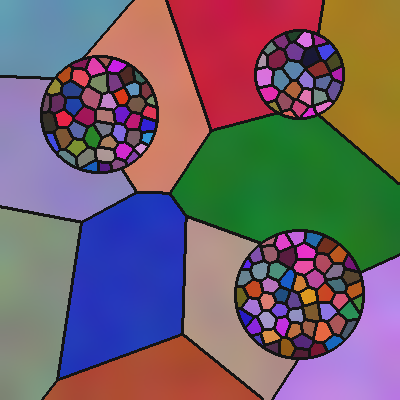
\includegraphics[width=20mm]{assets/drawn/grain-map-bimodal}};
    \node[anchor=west,label text] (fine) at (104,-21.4) {fine grains};
    \draw[udsdark,line width=0.4pt] (fine.west) -- ++(-1.6,0) -- (95,-21.15);
    \node[anchor=west,label text] (coarse) at (104,-28.4) {coarse grains};
    \draw[udsdark,line width=0.4pt] (coarse.west) -- ++(-1.6,0) -- (98,-26.9);
    \node[anchor=north west,card text,text width=63mm] at (80,-39.6)
      {\cardbullet{fine grains block dislocations: strength}
       \cardbullet{coarse grains let them glide: ductility}
       \cardbullet{the mismatch stores dislocations: hardening}};
  \end{tikzpicture}
  \note{\textbf{21:40--22:40}\par
    Left, patches of the initial alloys and patches generated for the candidates; the arrows mark what
      the authors call fine-grain regions (panel b).\par
    Below, the grain areas of all 2,000 original patches and of 400 generated ones, on a logarithmic
      axis: the generated patches have more grains in the smallest bin, at or below 0.4 µm² (panel d),
      which the authors read as a bimodal grain size.\par
    Their explanation: fine grains block dislocations and raise the strength, coarse grains leave room
      for them to glide and keep the ductility, and the mismatch between the two stores geometrically
      necessary dislocations (GNDs), which raise the strain hardening.\par
    The mechanism is established for heterogeneous microstructures; whether these generated patches
      show it remains to be checked.}
\end{frame}

% ------------------------------------------------------------ validation
\begin{frame}[source={Liao et al.\ (2026), Nat.\ Commun.\ 17, 11232, Fig.\ 5e, h (CC BY-NC-ND 4.0)}]
  {Simulation and one experiment}
  \begin{tikzpicture}[x=1mm,y=1mm]
    \useasboundingbox (0,0) rectangle (144,-54);
    \figpart{0}{0}{5}{1430}{49}{1908}{434}{54}
    \node[anchor=north west,label text,text width=54mm] at (0,-46.6)
      {new alloy, route from the literature: 60\,\% rolling at 1000\,°C, 5\,min at 850\,°C};
    \figpart{60}{0}{5}{660}{972}{2000}{1473}{84}
    \node[anchor=north west,label text,text width=84mm] at (60,-33.6)
      {candidate \candlabel{1}: i predicted, ii simulated by crystal plasticity (CPFE), iii measured on
       the new alloy};
  \end{tikzpicture}
  \note{\textbf{22:40--23:40}\par
    Two checks follow.\par
    First, crystal plasticity finite element (CPFE) simulations of two generated patches per candidate,
      with a slip model calibrated on three measured stress--strain curves; the Euler angles come from
      the pixel colours, the dislocation density from a learned mapping.\par
    Second, one experiment: an alloy processed by a route the authors chose from the literature to get
      a bimodal grain size, 60 percent hot rolling at 1000 °C and 5 minutes at 850 °C.\par
    Its EBSD map, left, shows coarse grains among many fine ones.\par
    Right, candidate 1 as predicted, simulated and measured: yield strength about 820, 805 and 825 MPa,
      elongation about 48, 44.5 and 43.5 percent, read from the bars.\par
    The paper concludes that the design is validated.}
\end{frame}
